\documentclass[lettersize,journal]{IEEEtran}
\usepackage{amsmath,amsfonts}
\usepackage{array}
\usepackage[caption=false,font=footnotesize,labelfont=sf,textfont=sf]{subfig}
\usepackage{textcomp}
\usepackage{graphicx}
\usepackage{booktabs}
\usepackage{url}
\usepackage{cite}
\usepackage{float}

\begin{document}

\title{Predicting Student Dropouts and Academic Successes}

\author{Alírio Rego, Nuno Vieira%
\thanks{Group project developed for the Introduction to Machine Learning course.}}

\markboth{Introduction to Machine Learning -- Final Project}{}

\maketitle

\begin{abstract}
Student dropout is a crucial challenge for higher education institutions and it is a product of various factors: not simply psychological ones like burnout, stress and anxiety but also socio-economic factors, insatisfaction with one's performance and a general lack of support by the instituions.
This project studies the use of supervised machine learning to predict whether a student is likely to drop out using these very factors and variables.

A preprocessing pipeline was built to handle numerical and categorical variables, and four classifiers were compared: Logistic Regression, Decision Tree, 
Random Forest and Support Vector Machine. The models were tuned using stratified cross-validation and evaluated on a test set using accuracy, 
macro-averaged precision, recall, F1-score, class-level metrics and confusion matrices. The project also discusses model limitations, overfitting and 
underfitting risks and the responsible use of predictive systems in education.
\end{abstract}

\begin{IEEEkeywords}
Student dropout, academic success, machine learning, classification, Random Forest, Logistic Regression, hyperparameter tuning.
\end{IEEEkeywords}

\section{Introduction}
\IEEEPARstart{E}{arly} identification of students who may be at risk can support timely interventions, such as academic tutoring, 
financial aid or personalized monitoring. Machine learning seems like a suitable approach for this type of problem because educational institutions 
often store valuable information about students that can be used to detect patterns related to their academic performance.

The objective of this project is to predict student dropout risk using a public tabular dataset. The original target variable has three classes: 
\emph{Dropout}, \emph{Enrolled}, and \emph{Graduate}. During the preliminary phase, the problem was treated as a supervised multiclass classification 
task. However, the results showed that the Enrolled class was consistently the most difficult to predict, by far. 
This class is also conceptually ambiguous, because it represents an intermediate academic state from which conclusions about the students' failure or 
success might be harder to draw, rather than a final academic outcome.

For the final version of the project, the problem was adapted into a binary classification task: \emph{Dropout} or \emph{Graduate}. 
Students labelled as Enrolled were removed from the dataset.

\section{Related Work}
Educational data mining and learning analytics have been widely studied as tools for predicting student performance, dropout risk and academic success. 
Rastrollo-Guerrero \emph{et al.} reviewed machine learning techniques for student performance prediction and showed that supervised learning methods are 
frequently used in this area \cite{rastrollo2020review}. Early warning systems are a common application of these techniques, since they aim to 
detect at-risk students before failure or dropout becomes irreversible.

Chung and Lee used Random Forest models for dropout early warning in high-school education and argued that predictive modeling can help identify students 
at risk in advance \cite{chung2019dropout}. In higher education, Realinho \emph{et al.} introduced the dataset used in this project, which was designed 
to support the prediction of dropout and academic success using information known at enrollment and at the end of the first two 
semesters \cite{realinho2022dataset}. The UCI Machine Learning Repository describes the original task as a three-category classification problem with 
student-level instances and 36 predictive features \cite{uci2021dropout}.

More recent comparative studies have explored several supervised learning algorithms on similar dropout prediction tasks. Villar and de Andrade compared 
Decision Tree, SVM, Random Forest and boosting algorithms, highlighting the importance of dealing with class imbalance and reporting F1-score for the 
different classes \cite{villar2024supervised}. Other work has also studied early warning systems in online learning contexts, emphasizing the need for 
interpretable and actionable predictions rather than purely automatic decisions \cite{baneres2023early}. These studies support the methodological 
choices adopted in this project: testing different model families, using class-sensitive metrics, and interpreting predictions cautiously.

\begin{figure}[!t]
\centering
\IfFileExists{fig_target_distribution.png}{\includegraphics[width=0.95\columnwidth]{fig_target_distribution.png}}{\fbox{\parbox{0.9\columnwidth}{\centering TODO: Insert target class distribution figure.}}}
\caption{Original target class distribution for Dropout, Enrolled, and Graduate.}
\label{fig:target_distribution}
\end{figure}

\begin{figure}[!t]
\centering
\IfFileExists{fig_feature_analysis.png}{\includegraphics[width=0.95\columnwidth]{fig_feature_analysis.png}}{\fbox{\parbox{0.9\columnwidth}{\centering TODO: Insert compact EDA figure, for example selected histograms or boxplots.}}}
\caption{Example exploratory analysis of relevant student features.}
\label{fig:feature_analysis}
\end{figure}

\section{Data Processing Pipeline}
A distinction was made between numerical variables and categorical variables and 
some categorical variables are represented by integer codes, but the numeric values do not necessarily represent meaningful ordinal 
relationships. Treating these variables as continuous values could introduce false assumptions, therefore, categorical variables were transformed using One-Hot Encoding.

Numerical variables were standardized with StandardScaler. This is especially relevant for Logistic Regression and Support Vector Machine, which are 
sensitive to the scale of the input variables. Tree-based models are less dependent on scaling, but a single preprocessing structure was maintained for 
consistency. The transformations were implemented using a ColumnTransformer and integrated into Pipelines.

The target variable was reformulated before training. Rows whose original target value was Enrolled were removed, since this class represents an 
intermediate and non-final state that introduces confusion. The remaining classes were converted into a binary target: Dropout and Graduate (Non-Dropout). 
The target labels were then encoded using Label Encoding. The data was split into training and test sets using an 80/20 stratified split with a fixed random seed. 

\section{Evaluation Strategy}
\subsection{Models and Parameter Tuning}
Four supervised classification algorithms were tested in order to compare different learning assumptions and levels of model complexity.

Logistic Regression was used as a sort of baseline. It is useful for checking whether the dataset contains patterns that can be captured by a relatively simple decision boundary.

Decision Tree was also chosen because it can capture nonlinear relationships and is easy to interpret. However, single trees can be unstable and prone to overfitting if they are too deep, or underfitting if they are too constrained.

Random Forest was included as a method that reduces the variance of individual decision trees by averaging many trees. This model is suitable for tabular data and can capture nonlinear relationships between variables.

Support Vector Machine was also tested because it is a strong classifier for structured data and can perform well when class separation is not purely linear. Both linear and RBF kernels were considered during tuning.

Hyperparameter tuning was performed with stratified 5-fold cross-validation on the training set and across all models. This ensured that the selected 
train-validation splits reflected the underlying class distribution, which as we've discussed is imbalanced.
GridSearchCV was used for Logistic Regression, Decision Tree, and SVM while RandomizedSearchCV was used for Random Forest due to the larger hyperparameter space.

The main optimization metric we selected was macro F1-score, which was done because the classes are not equally represented and because the goal is to 
avoid evaluating the model only by its performance on the majority class. In this problem, identifying Dropout students is especially important, so 
accuracy alone is not sufficient. Accuracy, macro precision, macro recall, macro F1-score, class-specific precision/recall/F1-score and confusion 
matrices were also used for final evaluation on the test set.

\begin{figure}[!t]
\centering
\IfFileExists{fig_hyperparameter_search.png}{\includegraphics[width=0.95\columnwidth]{fig_hyperparameter_search.png}}{\fbox{\parbox{0.9\columnwidth}{\centering TODO: Insert hyperparameter search visualization.}}}
\caption{Example hyperparameter search results using cross-validated macro F1-score.}
\label{fig:hyperparameter_search}
\end{figure}

\subsection{Results}
Tables I and II show that the reformulated binary task achieved substantially stronger performance than the original multiclass formulation. 
This time, SVM, Logistic Regression and Random Forest all performed very similarly. The best overall model was the tuned SVM, with an accuracy of 0.9146 and a macro F1-score of 0.9091. Logistic Regression achieved the same accuracy and a 
very similar macro F1-score of 0.9086, making it a strong alternative. Random Forest achieved slightly lower overall performance, 
with a macro F1-score of 0.9048, but obtained the highest Dropout precision. Decision Tree was clearly the weakest model, although it still achieved 
good enough performance.
Table~\ref{tab:model_comparison} presents the final test results for the tuned models.
\begin{table}[!t]
\caption{Final Model Comparison on the Binary Test Set}
\label{tab:model_comparison}
\centering
\footnotesize
\begin{tabular}{lcccc}
\toprule
Model & Acc. & Macro P & Macro R & Macro F1 \\
\midrule
SVM & 0.9146 & 0.9159 & 0.9041 & 0.9091 \\
Logistic Regression & 0.9146 & 0.9189 & 0.9015 & 0.9086 \\
Random Forest & 0.9118 & 0.9215 & 0.8949 & 0.9048 \\
Decision Tree & 0.8747 & 0.8696 & 0.8662 & 0.8678 \\
\bottomrule
\end{tabular}
\end{table}

\begin{table}[!t]
\caption{Class-Level F1-Scores on the Binary Test Set}
\label{tab:class_f1}
\centering
\footnotesize
\begin{tabular}{lcc}
\toprule
Model & Dropout & Graduate \\
\midrule
SVM & 0.8869 & 0.9314 \\
Logistic Regression & 0.8852 & 0.9320 \\
Random Forest & 0.8788 & 0.9307 \\
Decision Tree & 0.8378 & 0.8979 \\
\bottomrule
\end{tabular}
\end{table}

Compared with the preliminary multiclass formulation, the binary formulation is expected to reduce confusion because the ambiguous Enrolled class is no 
longer part of the target. This, however, does not make the problem trivial: the model still needs to distinguish students who dropped out from students 
who successfully graduated, and the class imbalance is still a factor. However, the final target is more meaningful because it compares two clearer academic outcomes and eliminates a limbo state.

\begin{figure}[!t]
\centering
\IfFileExists{confusion_matrix.png}{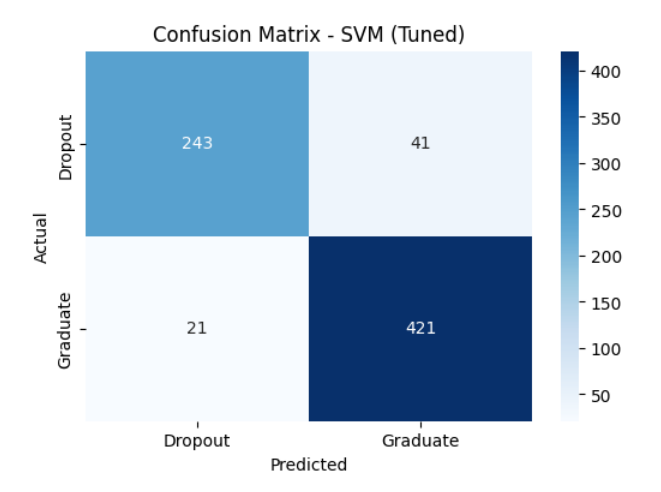
\includegraphics[width=0.95\columnwidth]{confusion_matrix.png}}{\fbox{\parbox{0.9\columnwidth}{\centering TODO: Insert final confusion matrix for the selected model.}}}
\caption{Confusion matrix for the selected model in the binary classification task.}
\label{fig:confusion_matrix}
\end{figure}

Looking at the confusion matrix for the SVM, false negatives correspond to students who actually dropped out but were predicted as Graduate. 
These errors are particularly serious because they may prevent timely intervention. As for false positives, they correspond to students predicted as Dropout even 
though they belong to the Graduate class. These errors may cause unnecessary intervention or concern, but they are usually less harmful than failing to identify a student who is genuinely at risk.

To take into account all of these differences, the final interpretation should consider macro F1-score, recall and the confusion 
matrix together. A useful model is not simply the model with the highest global accuracy, but the one that provides a good balance between detecting 
Dropout students and avoiding too many false alarms.

\subsection{Overfitting and Underfitting}
The comparison between models also helps discuss possible overfitting and underfitting behavior. Overfitting occurs when a model learns patterns that are 
too specific to the training data, including noise or accidental relationships, and therefore performs worse on unseen data. Underfitting occurs when a 
model is too simple or too constrained to capture the relevant relationships in the data, leading to poor performance on both training and test data.

Decision Trees can be prone to overfitting when they are too deep, because they may create very specific rules that separate the training examples almost 
perfectly but do not generalize well. For example, a deep tree could learn narrow combinations of student attributes that happen to appear in the 
training set but are not reliable indicators of dropout in general. On the other hand, if the tree is too restricted, for example by limiting its maximum 
depth too much or requiring too many samples per leaf, it may underfit by failing to capture important interactions between variables.

Random Forest reduces the overfitting risk of a single Decision Tree by training multiple trees and averaging their predictions. Since each tree is built 
using different samples and feature subsets, the final model is usually more stable and less sensitive to noise in the training data. However, Random 
Forests can still overfit if the individual trees are too complex and the dataset is small or noisy.

Logistic Regression is a simpler linear model, especially when regularization is used. This makes it less likely to overfit severely, but it can underfit 
if the true relationship between student variables and dropout is nonlinear or depends on complex feature interactions. Similarly, SVM models can 
generalize well when properly regularized, but their behavior depends on the kernel and hyperparameters. A linear SVM may underfit nonlinear patterns, 
while a highly flexible kernel configuration may overfit if not properly tuned.

The use of stratified cross-validation during hyperparameter selection reduced the risk of choosing a model that only performed well on a particular train-test split. 
However, without comparing training and validation performance directly, overfitting and underfitting cannot be confirmed with certainty. 
Further validation on external institutional data would also be necessary before considering real-world deployment.

\section{Responsible and Ethical Considerations}
Predicting academic outcomes has ethical consequences because model outputs may influence how students are perceived or supported. A model should not be used as an automatic decision-maker. Instead, it should be used as a decision-support tool that helps staff identify students who may benefit from additional support.

Fairness is a central concern. Some variables may be associated with socio-economic status, demographic characteristics, or access to resources. Even when sensitive attributes are not used directly for discrimination, other variables can act as proxies and reproduce existing inequalities. Therefore, any deployment of this type of model should include fairness monitoring and human review.

The cost of errors is also asymmetric. Failing to identify a student at risk may prevent timely intervention. However, incorrectly labeling a student as high risk may create stigma or unnecessary pressure. This is especially relevant in the binary formulation because the model directly separates students into Dropout and Non-dropout predictions. For this reason, predictions should be communicated carefully, used only to offer support, and combined with contextual information from teachers or academic services.

\section{Critical Analysis and Conclusions}
This project allowed us to apply the complete machine learning workflow to a realistic classification problem, from data understanding and preprocessing to model training, evaluation, and comparison. One of the main lessons learned was that model performance does not depend only on the algorithm chosen, but also on the quality of the data, the preprocessing decisions, the selected features, and the evaluation strategy. In the context of student dropout prediction, this is especially important because the problem is not only technical, but also has social and institutional implications.

During the development of the project, we observed that different models have different strengths and limitations. Simpler models, such as Logistic Regression, were easier to interpret and still achieved strong performance. This showed that more complex models are not always automatically better. On the other hand, models such as Random Forest and SVM were useful for capturing more complex patterns in the data, although they required more careful hyperparameter tuning. The Decision Tree model was easier to understand visually, but its lower performance also illustrated the risk of relying on a single tree, especially when the data contains complex relationships.

Another important aspect was the use of appropriate evaluation metrics. Accuracy alone was not sufficient to understand the quality of the models, particularly because dropout prediction can involve class imbalance and different costs for different types of errors. For example, failing to identify a student at risk of dropping out may be more serious than incorrectly flagging a student who is not actually at risk. Therefore, metrics such as precision, recall, and F1-score were essential to obtain a more complete view of model performance.

The project also highlighted the importance of avoiding overfitting and underfitting. Hyperparameter tuning and stratified cross-validation helped reduce the risk of selecting a model that only performed well on a specific train-test split. However, the results should still be interpreted with caution. Since the models were evaluated on a limited dataset, their performance may not fully represent how they would behave with data from other academic years, institutions, or student populations. External validation would be necessary before using such a model in a real decision-making context.

From a practical perspective, the project showed that machine learning can be a useful tool for supporting early identification of students at risk of dropout. However, it should not be used as the only basis for decisions. Predictions should be interpreted as decision-support information, not as definitive judgments about students. Human supervision is necessary to avoid unfair or incorrect interventions, especially because educational data may contain biases related to socioeconomic background, previous academic preparation, or institutional factors.

Overall, this work improved our understanding of supervised learning, classification models, model evaluation, and the importance of critical interpretation of results. It also made clear that building a machine learning model is not only about achieving the highest numerical score, but about understanding the problem, evaluating the model responsibly, and recognizing the limitations of the data and methodology used.

\section*{AI Tools Acknowledgement}
AI tools were used to support writing, organization, and critical review of the report. ChatGPT was used to help structure the document, identify missing 
sections, improve clarity, and review the consistency between the code, results, and written discussion. The final technical decisions, experiments, interpretation 
of results, and validation of the content were performed by the group. AI-generated suggestions were reviewed and adapted before inclusion.

\begin{thebibliography}{1}

\bibitem{rastrollo2020review}
J. L. Rastrollo-Guerrero, J. A. G\'{o}mez-Pulido, and A. Dur\'{a}n-Dom\'{i}nguez, ``Analyzing and predicting students' performance by means of machine learning: A review,'' \emph{Applied Sciences}, vol. 10, no. 3, p. 1042, 2020, doi: 10.3390/app10031042.

\bibitem{chung2019dropout}
J. Y. Chung and S. Lee, ``Dropout early warning systems for high school students using machine learning,'' \emph{Children and Youth Services Review}, vol. 96, pp. 346--353, 2019, doi: 10.1016/j.childyouth.2018.11.030.

\bibitem{realinho2022dataset}
V. Realinho, J. Machado, L. Baptista, and M. V. Martins, ``Predicting student dropout and academic success,'' \emph{Data}, vol. 7, no. 11, p. 146, 2022, doi: 10.3390/data7110146.

\bibitem{uci2021dropout}
M. V. Martins, D. Tolledo, J. Machado, L. M. T. Baptista, and V. Realinho, ``Predict Students' Dropout and Academic Success,'' UCI Machine Learning Repository, 2021, doi: 10.24432/C5MC89.

\bibitem{villar2024supervised}
A. Villar and C. R. V. de Andrade, ``Supervised machine learning algorithms for predicting student dropout and academic success: a comparative study,'' \emph{Discover Artificial Intelligence}, vol. 4, article 2, 2024, doi: 10.1007/s44163-023-00079-z.

\bibitem{baneres2023early}
D. Ba\~{n}eres, M. E. Rodr\'{i}guez-Gonzalez, and A. E. Guerrero-Rold\'{a}n, ``An early warning system to identify and intervene online dropout learners,'' \emph{International Journal of Educational Technology in Higher Education}, vol. 20, article 3, 2023, doi: 10.1186/s41239-022-00371-5.

\end{thebibliography}

\end{document}
